\section{Ajouter un poste client}(les champs de saisie marqu\'ees avec * doivent \^etre remplis correctement en tous cas)\\
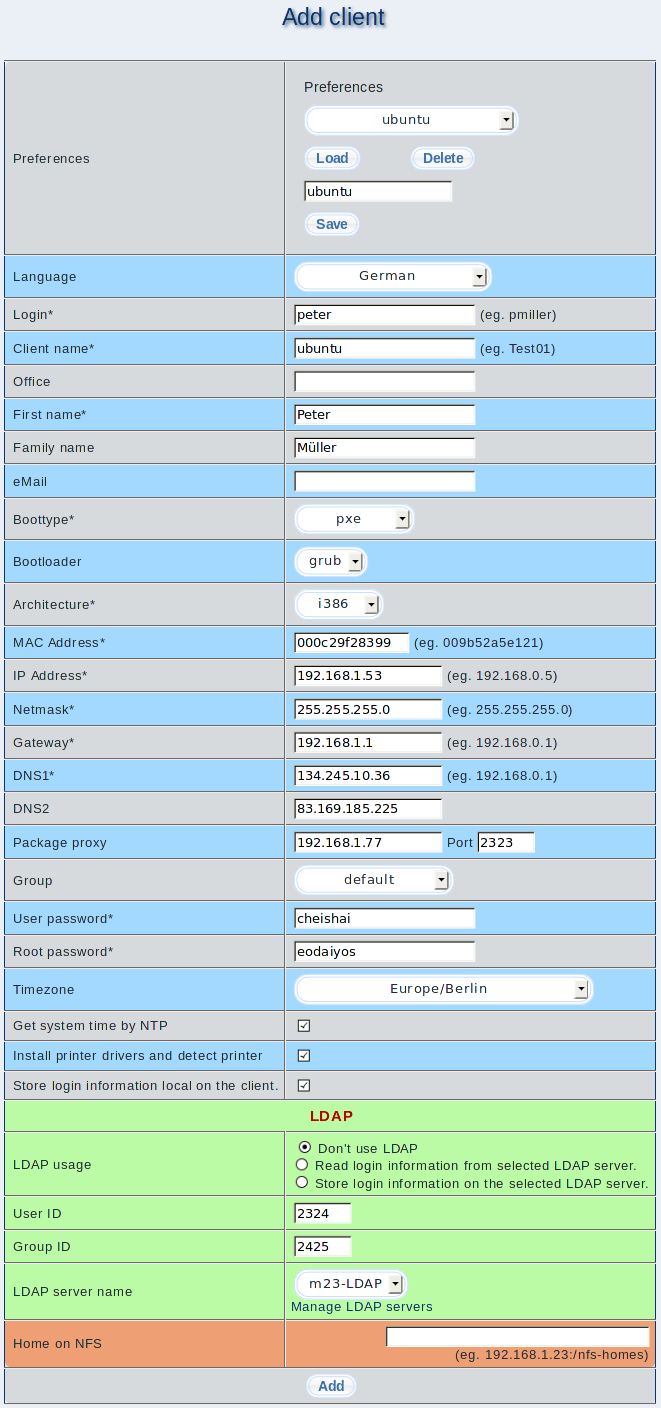
\includegraphics[scale=0.4]{/mdk/doc/manual/screenshots/fr/client_add.png} \\
\begin{itemize}
\item \textbf{Pr�f�rences:} Vous pouvez choisir entre des configurations d\'ej\`a enregistr\'ees et ensuite, vous avez la possibilit\'e de les charger o\`u de les effacer. Si vous voudriez enregistrer la configuration actuelle, entrez un nom pertinent et cliquez sur \textit{$\ll$Enregistrer$\gg$}.\\
\item \textbf{Langue:}Ici vous pouvez choisir la langue pour votre poste client m23. Cette langue sera employ\'ee pour l'ajustement du clavier, du bureau et de la console.\\
\item \textbf{Nom d'entr�e dans le syst�me:} Le nom pour l'entr\'ee dans le syst\`eme du poste client utilis\'e par l'utilisateur.\\
\item \textbf{Nom de poste client:} C'est le nom unique de votre client qui ne devrait pas \^etre employ\'e qu'une fois\\
\item \textbf{Section:} Cette information est volontaire, ici vous pouvez entrer o\`u le client se trouve (par ex. le num\'ero de la chambre etc.)\\
\item \textbf{Langue:} Ici vous pouvez choisir la langue pour votre client. Cette langue sera employ\'ee pour l'installation, pour tous les programmes install\'es, pour le clavier et les options de pays.\\
\item \textbf{Pr�nom:} Pr\'enom de l'utilisateur, correspond au nom d'entr\'ee dans le syst\`eme\\
\item \textbf{Nom de famille:} Nom de famille de l'utilisateur\\
\item \textbf{eMail:} Adresse de courrier \'electronique de l'utilisateur\\
\item \textbf{Type de boot:} Standard de d\'emarrage pour le d\'emarrage des clients vers le r\'eseau. (Notez: Si vous voudriez utiliser m23 avec un serveur DHCP existant, lisez la page suivante: externalDHCP)\\
\item \textbf{Chargeur d'amor�age:} Ici, choisissez quel chargeur d'amor\c{c}age/boot loader vous voudriez utiliser pour l'amor\c{c}age du noyau Linux et des autres syst\`emes d'exploitation eventuellement install\'es. Vous pouvez choisir entre LILO (LInux LOader) et GRUB (GRand Unified Bootloader).\subsection{Information suppl\'ementaire}
La manipulation des param\`etres de d\'emarrage par des personnes non autoris\'ees est emp\^ech\'ee par la protection avec un mot de passe \`a partir de la version m23 0.6.4 . Il est n\'ecessaire d'entrer le mot des passe de d\'emarrage du r\'eseau. Vous pouvez l'extraire dans le centre de contr\^ole sous \textit{$\ll$Connexion directe au poste client$\gg$}.\\
\item \textbf{Architecture du processeur:} Ici, vous pouvez choisir si vous voudriez installer le logiciel pour la version 32 bits ou 64 bits. Regardez aussi le renseignement en bas de la page.\\
\item \textbf{Adresse MAC:} Adresse MAC de la carte r\'eseau du client (par ex. 00:D0:B7:23:86:5C)\\
\item \textbf{Adresse IP:} Adresse IP souhait\'ee du client (par ex. 192.168.1.23)\\
\item \textbf{Masque r�seau:} Masque r\'eseau du r\'eseau (par ex. 255.255.255.0)\\
\item \textbf{Passerelle:} IP de la passerelle pour les connections \`a l'internet ou des autres connections hors du r\'eseau\\
\item \textbf{DNS1:} Adresse IP du serveur DNS pour dissoudre les noms d'internet\\
\item \textbf{DNS2 (facultatif):} Adresse IP du serveur DNS backup\\
\item \textbf{Proxy des paquets:} Le poste client essaie de t\'el\'echarger les paquets de logiciel du num\'ero IP du serveur proxy indiqu\'e. Dans le cas g\'en\'eral, il s'agit du num\'ero IP du serveur m23, mais on peut aussi entrer le num\'ero d'un autre serveur proxy. Si vous laissez ce champs de saisie vide, le client va t\'el\'echarger les paquets de logiciel de l'internet. Entrez \'egalement l'adresse du port du serveur proxy. Au cas du serveur m23, c'est le port 2323. Quand vous ouvrez le dialogue \textit{$\ll$Ajouter un client$\gg$}, le serveur m23 est indiqu\'e comme serveur proxy de standard.\\
\item \textbf{Groupe (facultatif):} Nom du groupe de postes client \`a laquelle appartient le poste client\\
\item \textbf{Mot de passe de l'utilisateur:} C'est le mot de passe de l'utilisateur employ\'e pour la premi\`ere entr\'ee dans le syst\`eme. Ce mot de passe consiste de six chiffres choisis par hasard, mais vous pouvez aussi choisir un autre mot de passe.\\
\item \textbf{Mot de passe de la racine:} C'est le mot de passe qui est employ\'e pour l'acc\`es root au client. Il consiste de huit chiffres choisis par hasard, mais vous pouvez aussi choisir un autre mot de passe.\\
\item \textbf{Fuseau horaire:} Ici, vous pouvez d\'efinir le fuseau horaire, que le poste client doit utiliser.\\
\item \textbf{D�terminer l'heure syst�me par NTP:} S\'electionnez cette option quand vous voudriez que l'heure du poste client doit \^etre accord\'ee par l'internet.\\
\item \textbf{Installer les pilotes de l'imprimante et d�tecter l'imprimante:} Quand vous s\'electionnez cette option, des pilotes d'imprimante seront install\'es et les imprimantes connect\'ees seront d\'etect\'ees.\\
\item \textbf{Enregistrer les donn�es d'ouverture de session local sur le poste client.:}Mettez un crochet ici pour pouvoir utiliser l'entr\'ee dans le syst\`eme locale des postes client.\\
\item \textbf{Ne pas utiliser le LDAP}: Pour pouvoir utiliser l'entr\'ee dans le syst\`eme locale des postes client comme seule option, choisissez \textit{$\ll$Ne pas utiliser le LDAP$\gg$}. \\
\item \textbf{Lire les donn�es d'ouverture de session du serveur LDAP s�lectionn�.}: Si vous voudriez utiliser les donn\'ees d'authentification d'utilisateur enregistr\'ees sur le serveur LDAP, cliquez sur \textit{$\ll$Lire les donn�es d'ouverture de session du serveur LDAP s�lectionn�.$\gg$}.\\
\item \textbf{Enregistrer les donn�es d'ouverture de session sur le serveur LDAP.}: Mais si vous choisissez d'entrer les donn\'ees d'utilisateur indiqu\'ees en haut dans la banque de donn\'ees LDAP du serveur m23 et de les utiliser pour l'entr\'ee dans le syst\`eme sur les postes client, s\'electionnez \textit{$\ll$Enregistrer les donn�es d'ouverture de session sur le serveur LDAP.$\gg$}. Pour pouvoir s\'electionner cette option, il vous faut d'un serveur LDAP avec acc\`es complet, comme les donn\'ees indiqu\'ees en haut seront enregistr\'ees sur le serveur LDAP.\\
\item \textbf{ID de l'utilisateur, ID du groupe}: En plus, vous devez choisir l'\textit{$\ll$ID de l'utilisateur$\gg$} et l'\textit{$\ll$ID du groupe$\gg$} pour l'utilisateur. Ceci est important surtout quand vous voudriez utiliser NFS pour l'enregistrement des r\'epertoires personnels.\\
\item \textbf{Nom du serveur LDAP}: Enfin, vous devez s\'electionner un serveur LDAP de la liste chez \textit{$\ll$Nom du serveur LDAP$\gg$}. Si le serveur LDAP souhait\'e n'y serait pas affich\'e, vous pouvez l'ajouter apr\`es un clic sur \textit{$\ll$Administrer le serveur LDAP$\gg$}.\\
\item \textbf{R�pertoire personnel sur le serveur NFS:} Cette option assure que les donn\'ees d'utilisateur seront enregistr\'ees sur un serveur NFS central, pour qu'elles puissent \^etre acc\'ed\'ees de tout poste client (en combination avec LDAP). Pour activer le NFS, entrez le nom de l'ordinateur ou son adresse IP et le chemin pour l'enregistrement des r\'epertoires personnels, comme par exemple: \\
\begin{verbatim}
192.168.1.42/nfs/home
\end{verbatim}
.\\
\end{itemize}
Veuillez ajouter le client en cliquant sur \textit{$\ll$Ajouter$\gg$}.\\
\subsection{Information suppl\'ementaire:}
Apr\`es \^etre \'etabli, le client parcourt une sequence de d\'etection du mat\'eriel, pendant laquelle des informations, comme par ex. sur la taille du disque dur utilis\'e, sont envoy\'ees au serveur.\\
Apr\`es l'ach\`evement du transfert des donn\'ees l'\'etat du client change \`a \textit{$\ll$jaune$\gg$} et vous pouvez ajuster le client. Pour cela, cliquez sur \textit{$\ll$Postes clients$\gg$} et puis sur \textit{$\ll$Configuration$\gg$} dans le menu.\\
\subsection{Renseignement concernant l'architecture du processeur}
m23 est compatible avec les processeurs 32 et 64 bits. Une version 32 bits peut \^etre install\'ee sur un ordinateur avec 64 bits, \`a l'envers, ce n'est pas possible. Pour profiter du potential entier d'un microprocesseur 64 bits, vous devriez choisir \textit{$\ll$amd64$\gg$}. Parmi la cat\'egorie \textit{$\ll$amd64$\gg$} ne comptent pas seulement les CPUs de AMD, mais aussi ceux de Intel.fallen nicht nur die CPUs von AMD sondern auch die von Intel. Par exemple, les CPUs des Intel Pentium D, Pentium Extreme Edition, Celeron D et Core 2 et les CPUs AMD Sempron, Athlon 64, Athlon X2 et Phenom y appartiennent.\\
